\documentclass[border=8pt]{standalone}
\usepackage{tikz}
\usepackage{amsmath}
\usepackage{amssymb}
\usepackage[scaled=0.92]{helvet}\renewcommand\familydefault{\sfdefault}
\usetikzlibrary{positioning,fit,backgrounds,calc,arrows}

\definecolor{inF}{RGB}{226,233,241}\definecolor{inL}{RGB}{70,90,112}
\definecolor{reF}{RGB}{255,238,208}\definecolor{reL}{RGB}{196,138,38}
\definecolor{eF}{RGB}{214,229,247}\definecolor{eL}{RGB}{38,92,164}
\definecolor{dF}{RGB}{209,238,231}\definecolor{dL}{RGB}{26,132,118}
\definecolor{tF}{RGB}{230,221,243}\definecolor{tL}{RGB}{114,70,162}
\definecolor{cF}{RGB}{219,238,219}\definecolor{cL}{RGB}{56,140,60}
\definecolor{emF}{RGB}{249,225,225}\definecolor{emL}{RGB}{178,68,68}
\definecolor{arr}{RGB}{70,78,90}

\begin{document}
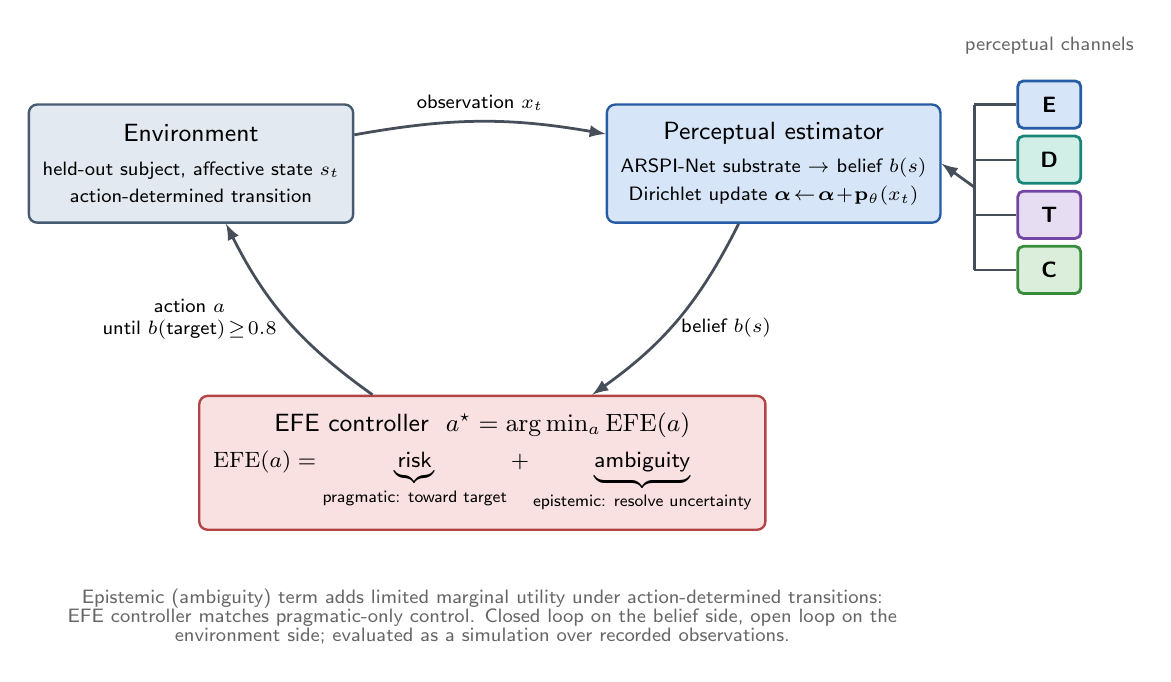
\begin{tikzpicture}[
  font=\small,
  box/.style={rounded corners=3pt, draw, line width=0.85pt, align=center, inner sep=5pt, minimum height=15mm, minimum width=40mm},
  env/.style={box, fill=inF, draw=inL},
  perc/.style={box, fill=eF, draw=eL},
  efe/.style={box, fill=emF, draw=emL, minimum height=17mm},
  mini/.style={rounded corners=2pt, draw, line width=1pt, minimum width=8mm, minimum height=6mm, font=\footnotesize\bfseries, inner sep=1pt},
  flow/.style={->, >=latex, line width=1pt, draw=arr},
]

% ---- cycle nodes (clockwise): env -> perception -> efe -> env ----
\node[env]  (env)  at (0,3.4)    {Environment\\[1pt]{\scriptsize held-out subject, affective state $s_t$}\\[-1pt]{\scriptsize action-determined transition}};
\node[perc] (perc) at (7.4,3.4)  {Perceptual estimator\\[1pt]{\scriptsize ARSPI-Net substrate $\rightarrow$ belief $b(s)$}\\[-1pt]{\scriptsize Dirichlet update\ $\boldsymbol{\alpha}\!\leftarrow\!\boldsymbol{\alpha}\!+\!\mathbf{p}_{\theta}(x_t)$}};
\node[efe]  (efe)  at (3.7,-0.4) {EFE controller\ \ $a^\star=\arg\min_a\mathrm{EFE}(a)$\\[2pt]{\footnotesize $\mathrm{EFE}(a)=\underbrace{\text{risk}}_{\text{pragmatic: toward target}}+\underbrace{\text{ambiguity}}_{\text{epistemic: resolve uncertainty}}$}};

% ---- loop arrows ----
\draw[flow] (env) to[bend left=10] node[above,font=\scriptsize]{observation $x_t$} (perc);
\draw[flow] (perc) to[bend left=14] node[right,font=\scriptsize,align=left,pos=0.55]{belief $b(s)$} (efe);
\draw[flow] (efe) to[bend left=14] node[left,font=\scriptsize,align=center,pos=0.5]{action $a$\\{\scriptsize until $b(\text{target})\!\ge\!0.8$}} (env);

% ---- perceptual channels feeding the estimator ----
\node[mini,fill=eF,draw=eL] (mE) at (10.9,4.15){E};
\node[mini,fill=dF,draw=dL] (mD) at (10.9,3.45){D};
\node[mini,fill=tF,draw=tL] (mT) at (10.9,2.75){T};
\node[mini,fill=cF,draw=cL] (mC) at (10.9,2.05){C};
\node[font=\scriptsize,align=center,text=black!60] at (10.9,4.9){perceptual channels};
\coordinate (mrail) at (9.95,3.1);
\draw[line width=0.85pt,draw=arr] (9.95,4.15) -- (9.95,2.05);
\draw[line width=0.85pt,draw=arr] (mE.west) -- (mE.west -| mrail);
\draw[line width=0.85pt,draw=arr] (mD.west) -- (mD.west -| mrail);
\draw[line width=0.85pt,draw=arr] (mT.west) -- (mT.west -| mrail);
\draw[line width=0.85pt,draw=arr] (mC.west) -- (mC.west -| mrail);
\draw[flow] (9.95,3.1) -- (perc.east);

% ---- honest finding + scope note ----
\node[font=\scriptsize,align=center,text=black!60] at (3.7,-2.35)
  {Epistemic (ambiguity) term adds limited marginal utility under action-determined transitions:\\[-1pt]EFE controller matches pragmatic-only control. Closed loop on the belief side, open loop on the\\[-1pt]environment side; evaluated as a simulation over recorded observations.};

\end{tikzpicture}
\end{document}
